\documentclass{article}
\usepackage{amsmath}
\usepackage{enumitem}
\usepackage{graphicx}
\begin{document}
\title{Dilations: Question 37}
\author{Ana Bhattacharjee}
\date{\today}
\maketitle{}
\begin{center}
\begin{figure}[!htbp]
  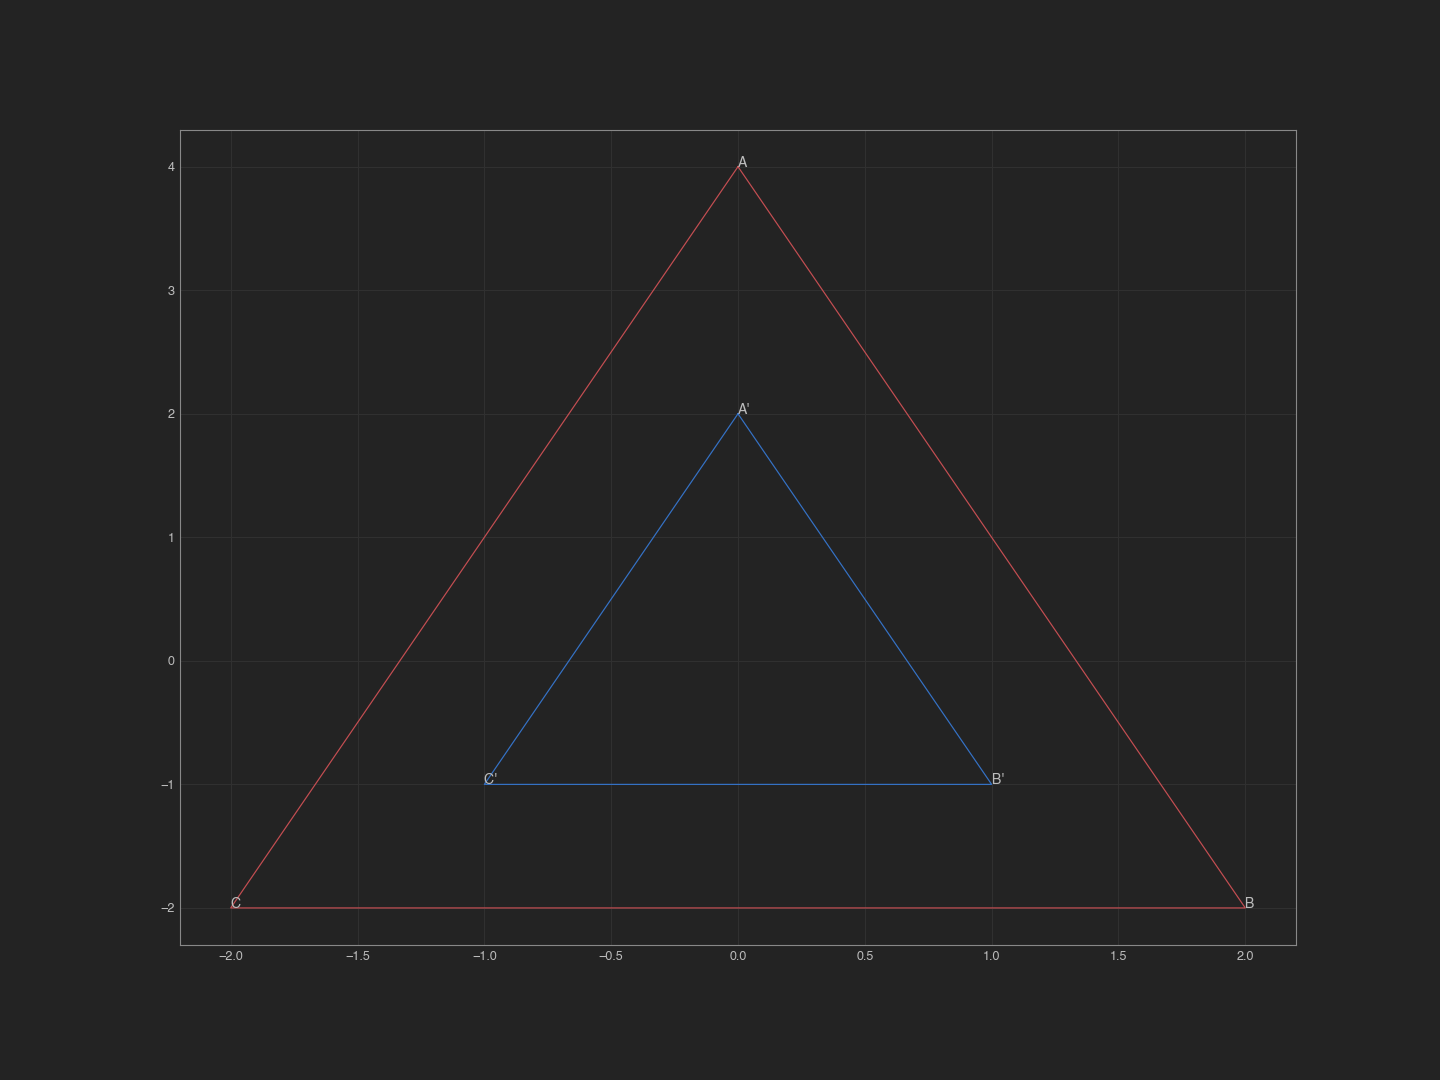
\includegraphics[width=1.0\columnwidth]{../q37}
  \caption{Triangle with Dilation}
\end{figure}
\begin{enumerate}[label=(\alph*)]
  \item The sides of the image will be half of the sides of the pre-image.
  \item The orientations of the side will be parallel to each other.
  \item The corresponding angles will be congruent by their measures. 
\end{enumerate}
\end{center}
\end{document}
